\author[Roy Stegeman]{}
\institute{University of Milan}
\subsection{Methodology correlations}

\begin{frame}{Self-correlation of PDF sets}
    	\begin{columns}[t]
        	\column{0.5\linewidth}
        	
		 Are PDF sets based on the same NNPDF methodology and underlying data fully correlated?

        	\vspace{0.2cm}

		\textit{We calculate the correlation using PDF pairs fitted to the same data replicas.}
        	
        	\vspace{0.2cm}

			No, they are not fully correlated as a result of uncorrelated functional uncertainties.

		\vspace{0.2cm}
			\only<2>{If the correlation is higher, this means the functional uncertainty is smaller if compared to the data uncertainty.}

        	\column{0.5\linewidth}
        		\begin{center}
        		\begin{figure}
            		\captionsetup{format=smol}
            		\includegraphics<1>[width=\textwidth]{roy_pdf_correlations/nnpdf31_corr.pdf}
            		\includegraphics<2>[width=\textwidth]{roy_pdf_correlations/nnpdf31&40_corr.pdf}
            		\vspace{-0.9cm}
            		\caption{\tiny PDF-PDF self-correlation between two PDF sets based on the same NNPDF methodology and data, but different (random) initialization. }        		
			\end{figure}
			\end{center}

    	\end{columns}
\end{frame}


\begin{frame}{Combination of PDF sets}
    	\begin{columns}[t]
        	\column{0.6\linewidth}

			At present the PDF4LHC combination method is a simple averaging. 

        	\vspace{0.2cm}

			Can we achieve a more precise results by including underlying correlations?

        	\vspace{0.2cm}

			No, this can lead to arbitrarily small uncertainties.

       	\column{0.4\linewidth}
       	\vspace{-1.5cm}
       	\begin{center}
       		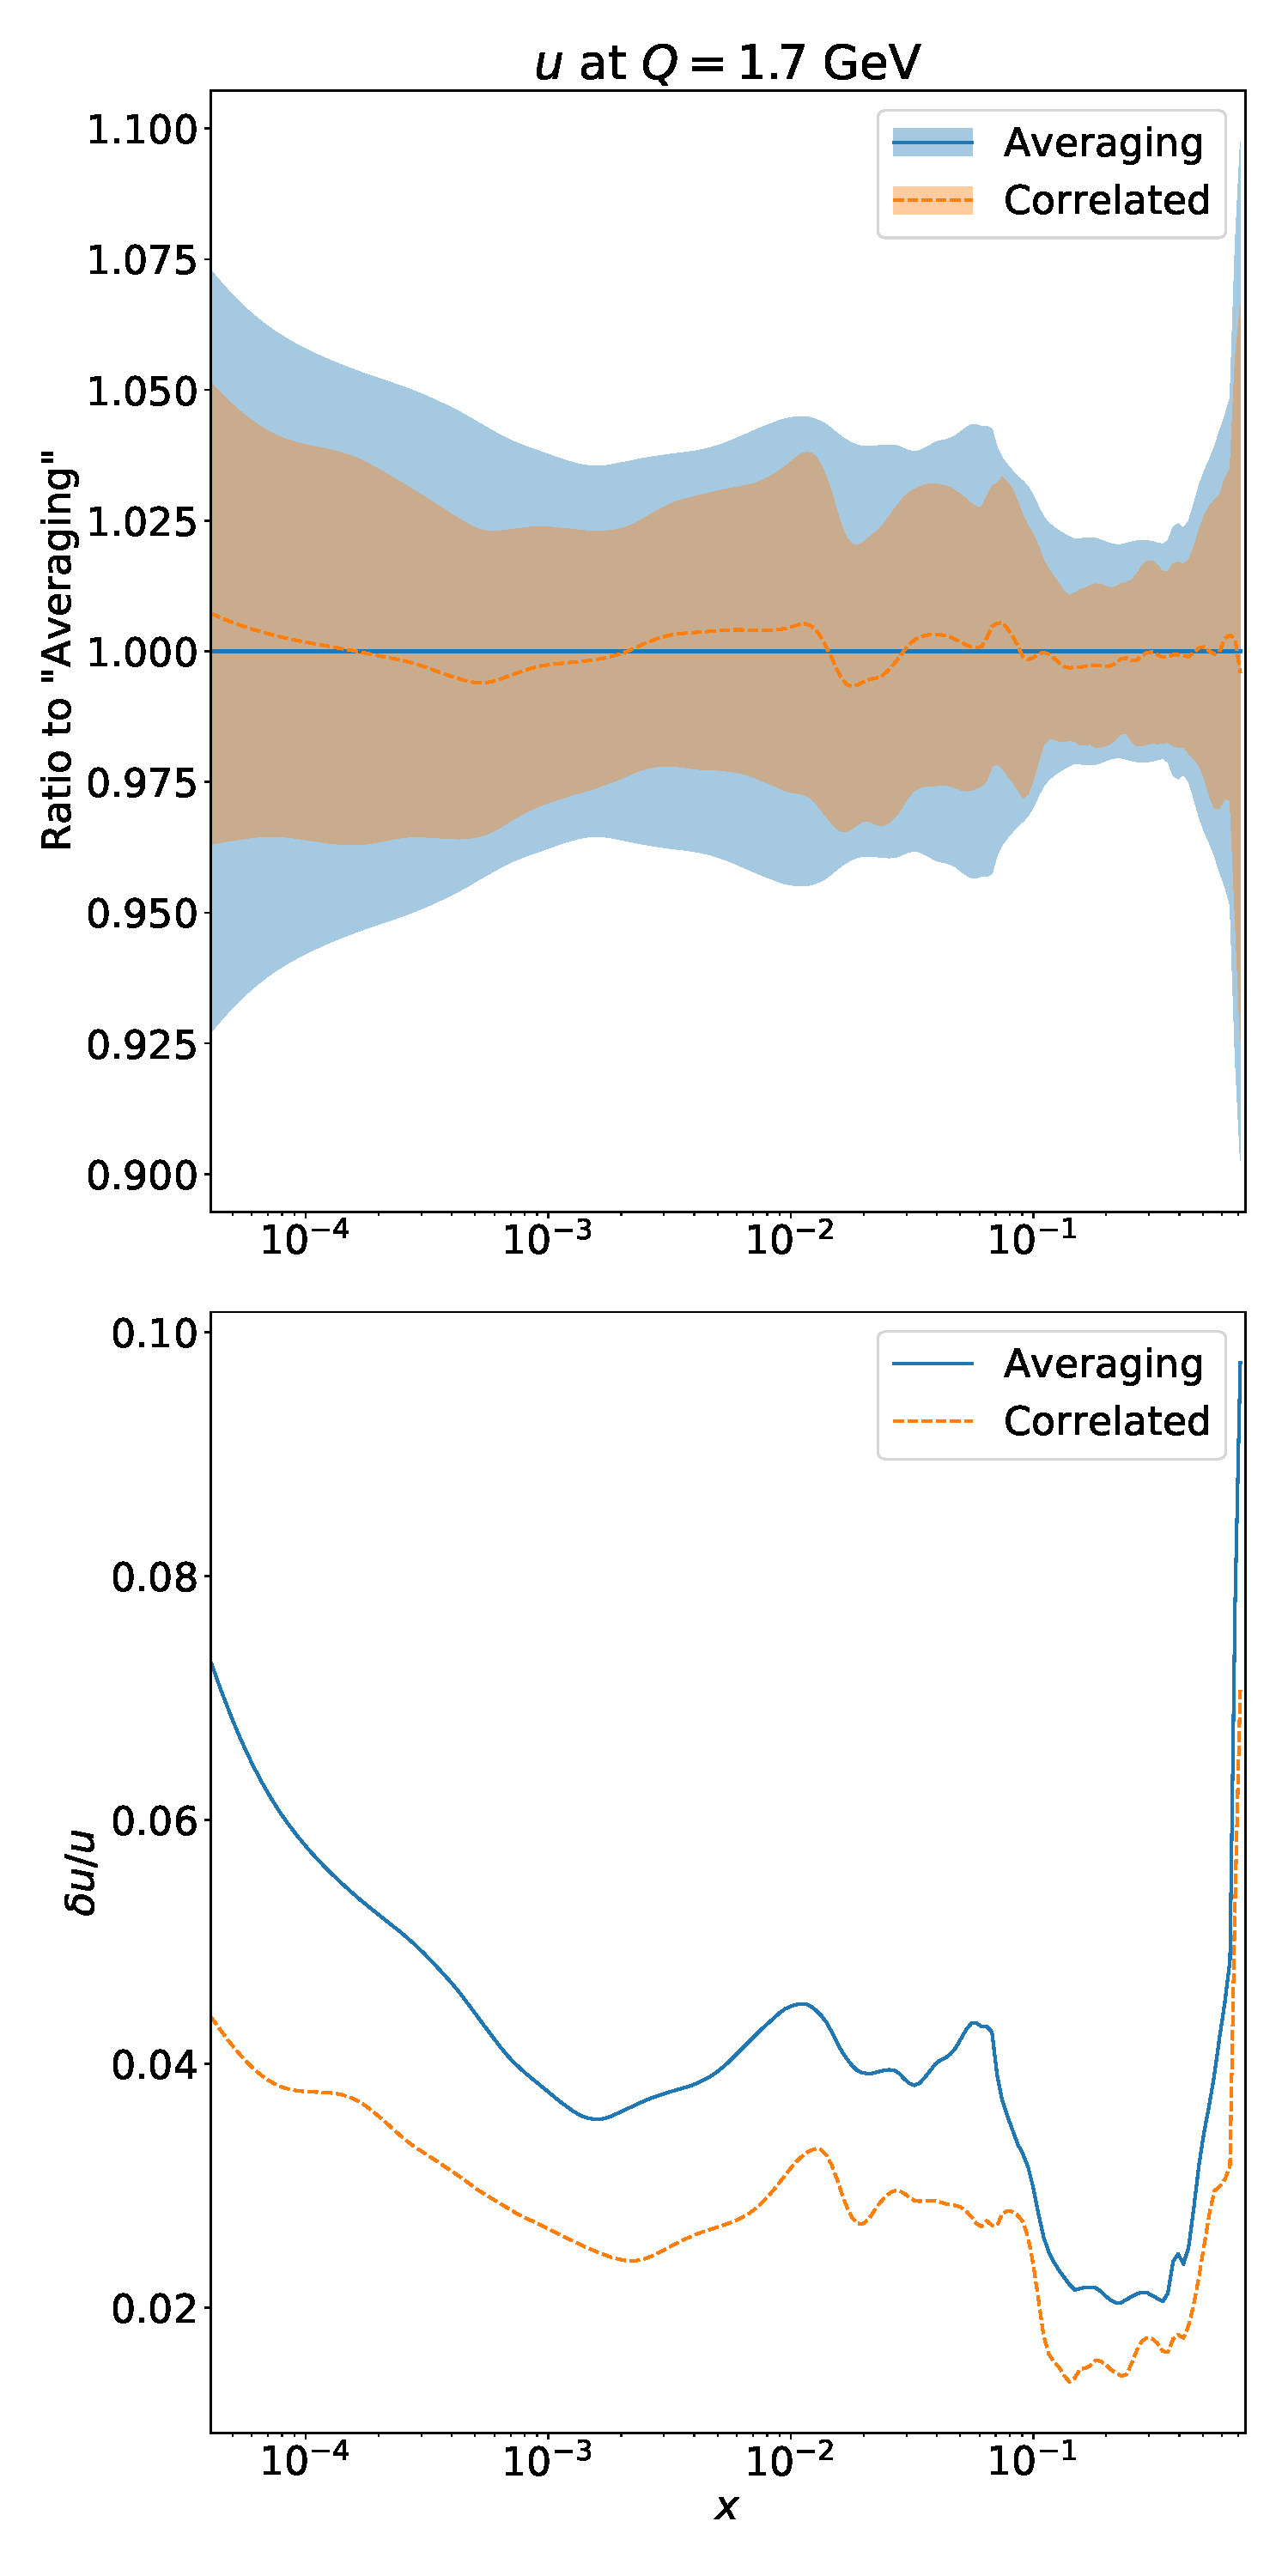
\includegraphics[height=1\textheight]{roy_pdf_correlations/ratio_2.pdf}
       	\end{center}
			
    	\end{columns}
\end{frame}
